\section{\centerline{Methodology}}
\label{sec:methodology}


\vspace {15pt}
The aim of this project is to investigate the capability of EEG signals in providing reliable information for the detection of the user’s intent, when using a single electrode connected to the Fp1 position of the scalp. To achieve this experimentally, it is necessary to (a) setup the necessary equipment to facilitate the recordings of the EEG signals, (b) device the experiments that will enable the collection of appropriate data and (c) to specify the methodology to analyse the collected signals in order to complete the investigation and reach to a conclusion. An overview of the methodology to be used is shown in Figure \ref{overview}. As shown in Figure  \ref{overview}, the first part of the methodology concerns a closed loop BCI system where the EEG signals are amplified, sampled and stored in a computer file, while the spectrum of the EEG signal is displayed on the screen. The subject observes the spectrum and use it as a feedback of the effect of his/her effort. The second part concerns the analysis of the recorded EEG signal. This includes the pre-processing of the signal, the investigation on the effect of the spectrum of the alpha band frequencies and the calculation of the SNR. 

\begin{figure}[hbt!]
	\centering
	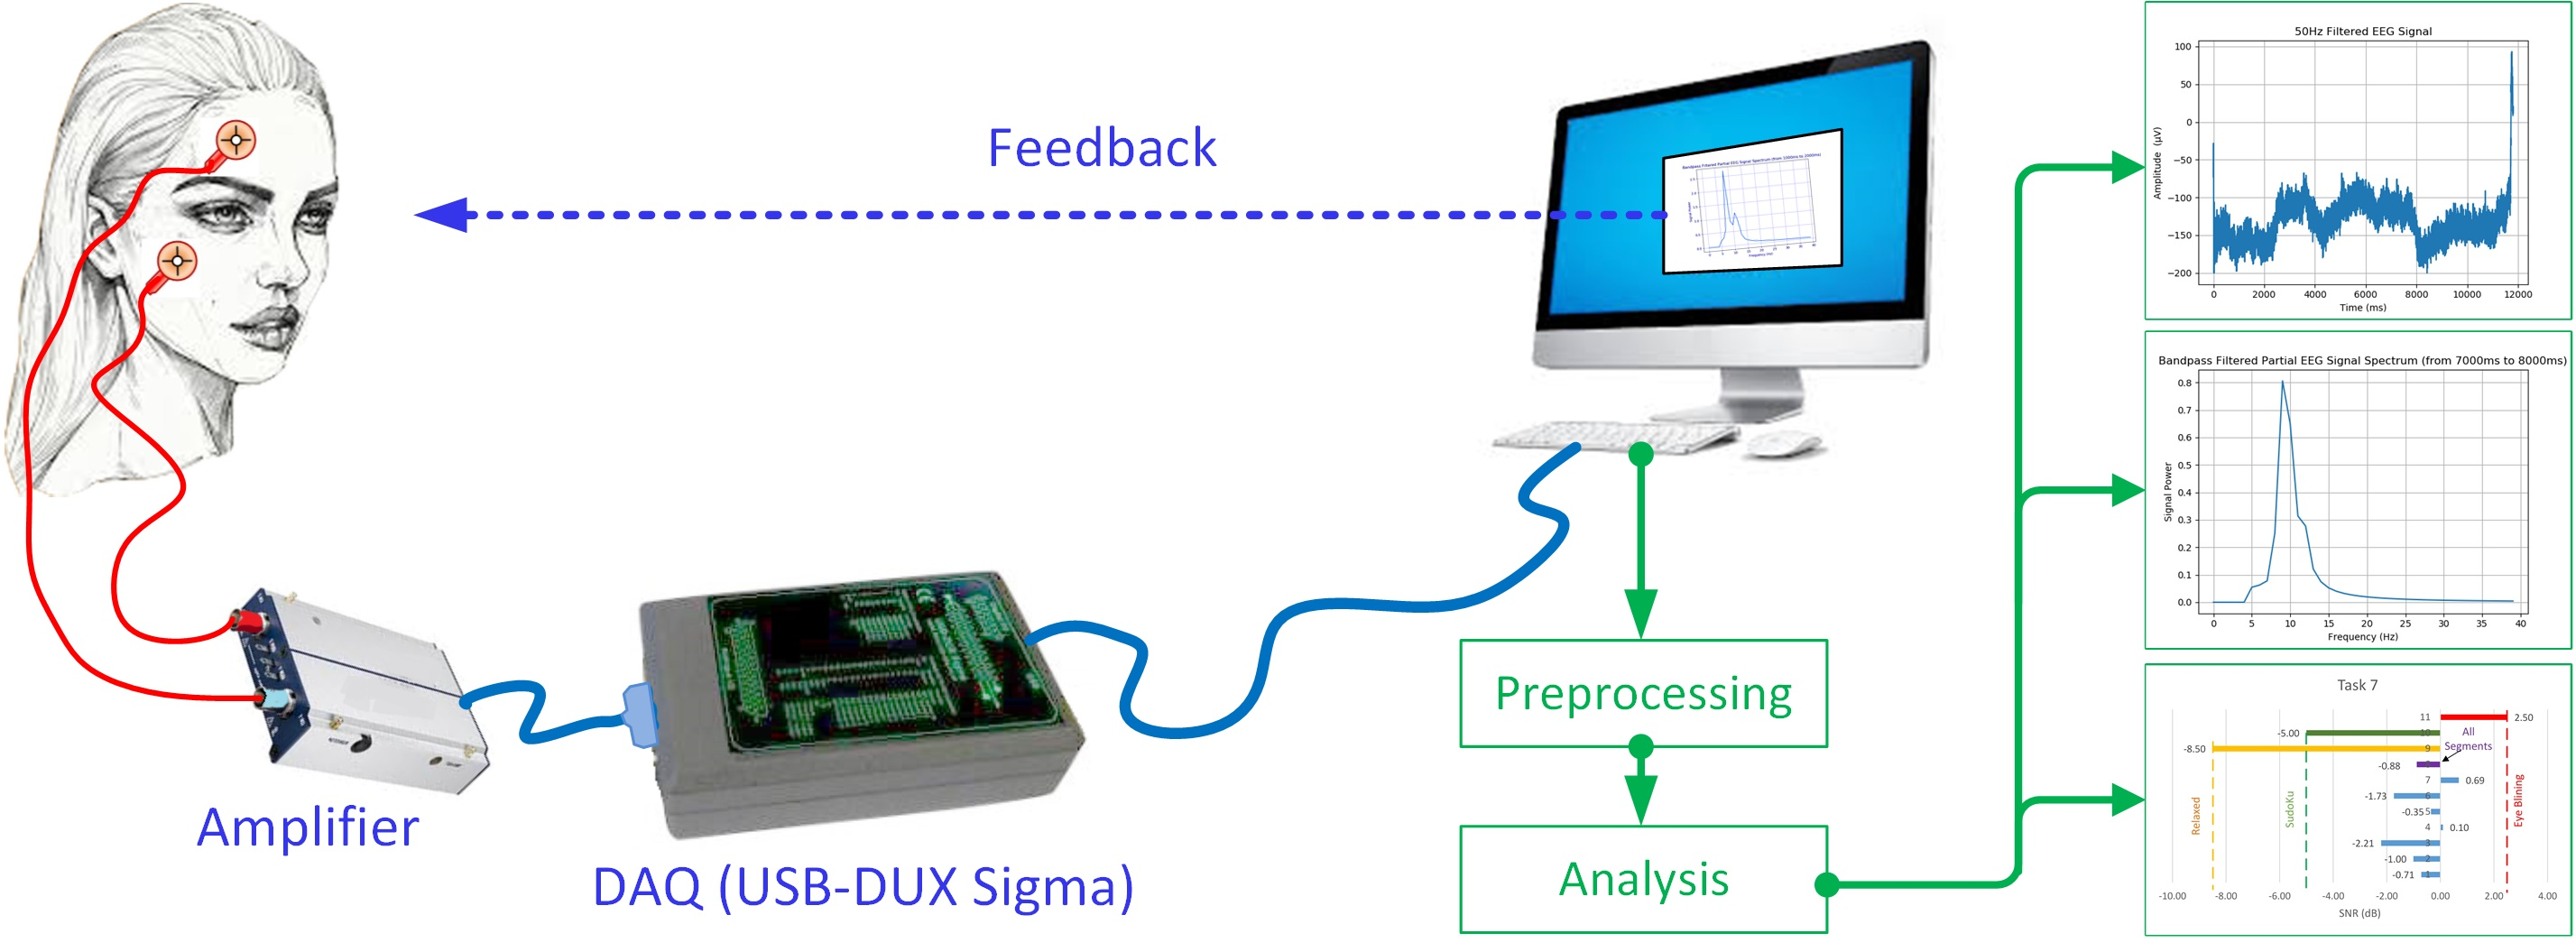
\includegraphics[width=\linewidth]{Figures/Overview.jpg} 
%	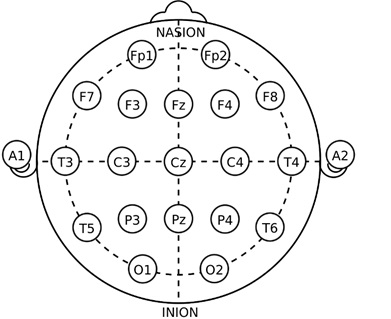
\includegraphics[width=8cm]{Figures/Brain_I20.jpg} 
	\caption{Methodology Overview} 
	\label{overview} 
\end{figure}

\subsection{\bf{Experimental Setup:}}
The hardware needed for the recording of EEG signals includes the EEG electrodes, the signal amplifier, the data acquisition hardware (Data converter board) and a computer. The diagram for the experimental setup is shown in Figure \ref{Hsetup}.

\begin{figure}[hbt!]
	\centering
	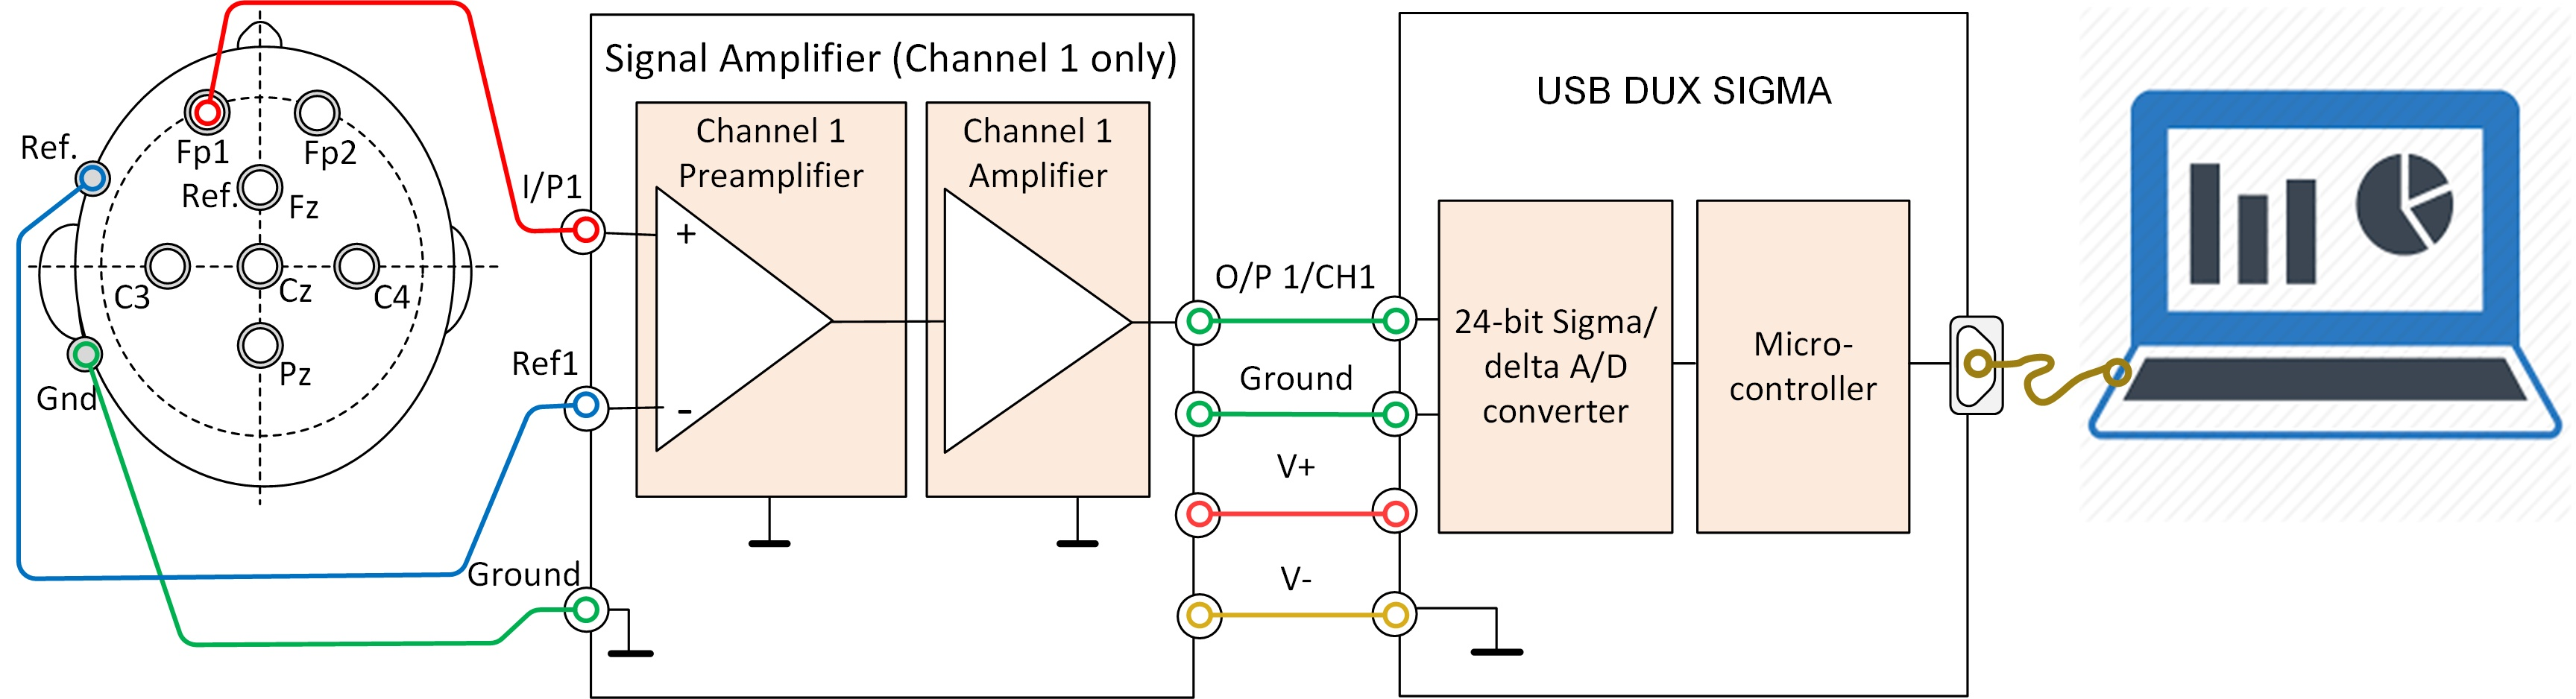
\includegraphics[width=\linewidth]{Figures/HardwareSetup.jpg} 
%	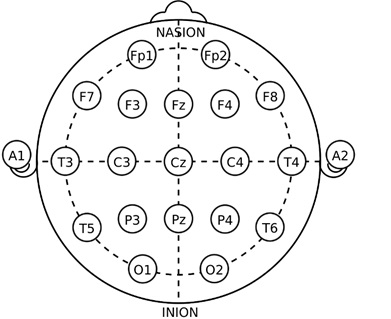
\includegraphics[width=8cm]{Figures/Brain_I20.jpg} 
	\caption{Block Diagram of the Experimental Setup} 
	\label{Hsetup} 
\end{figure}

Three disposable EEG electrodes are attached on the skin at the subject’s head area. The signal electrode is attached on the Fp1 position, the reference electrode is attached on the cheek and the ground is attached on the back of the ear of the subject. The EGG electrodes are kept in place by means of a hat that has the functionality of an EEG cap. 

The EEG signals are amplified by a custom made amplifier. This is a two-channel amplifier. The experiments were conducted using only one of the two channels. The gain of the amplifier is specified by two internal resistances and is set to be equal to 50. The voltage swing of the amplifier is from -5V to +5V. The signal amplifier is attached on a hat placed on the head of the subject. 

The output of the amplifier is connected to one of the analogue input channels of the data acquisition unit. This used is the “USB DUX SIGMA” 24-bit analogue-to-digital converter board (Porr, and linux-usb-daq.co.uk). This board has 16 analogue input channels with a maximum input voltage swing of -1.33V to +1.33V. The sampling frequency is 1KHz. Care must be taken in order not to exceed the maximum input voltage swing, because in such a case, the input signal will be clipped and behave like a square waveform with higher frequency harmonics.  The data acquisition unit provides also the supply voltage for the signal amplifier. The data acquisition unit is connected to a host computer through a USB cable. 

EEG recordings were made using the open source software “Comedirecord” \citep{Porr}. This software enables the acquisition of signals, signal filtering, display of time domain signal, display of the frequency spectrum and the recording of the raw signal.

\subsection{\bf{Experiment Procedure:}}
To investigate the EEG signals in the alpha wave frequency band taken from an electrode connected to the Fp1 position and the achieved SNR, experiments are required to be done with willing participants referred to as the subjects. During these experiments the subjects will be asked to perform a mental task. The EEG signals generated by the subject will be recorded on a computer, while the screen of the computer will display the real time frequency spectrum of the EEG signal. This will enable a closed loop control of the BCI system. The subjects will be asked to look at their own Fourier spectrum and try to consciously maximize the alpha band frequency peak, thus achieving maximum SNR.  

The mental tasks to be carried out by the subjects was set in such a way to avoid any body movement by the subject, such as using a pen and paper to solve a complex mathematical expression, and thus limit as much as possible artefacts. Furthermore, trying to solve a complex mathematical expression while at the same time observing the spectrum on the screen of the computer is a very difficult task to accomplish. Therefore, the experiments were carried out using the following two mental tasks. 

\begin{description}
 	\item[Task1:] 	The subject is asked to concentrate on the window displaying the Fourier spectrum of the generated EEG and try to consciously move it, either vertically or horizontally, while observing the generated alpha band peak, and try to maximize it. Trying to move an object like a cursor on the screen of a computer is a task employed in a number of BCI research projects  \citep{Wolpaw2004}. 
	\item[Task2:]	The subject is asked to concentrate on the window displaying the Fourier spectrum of the generated EEG signal and try to consciously maximize the 10Hz peak. Optionally, the subject is asked to do the same for other frequencies such as 20Hz or 30Hz. The ability to achieve this needs to be checked, since each frequency band reflects different types of brain activities that might not be relevant to the specific intent of the subject.    
\end{description}

The ability to consciously produce EEG signals varies from person to person. Due to the nature of the experiments, the subjects are preferably required to have a background in engineering. Still, it might be hard for people to be able to do this experiment accurately without first trying out the system. Therefore, a training session for each subject is conducted before the actual experiments, in order to familiarize the subject with the system and the expected mental tasks. The duration for each training session is about 30 minutes and includes the following:

\begin{enumerate}
 	\item The subject is introduced to the purpose of this work and the experiments himself. 
 	\item	The subject is asked to do different body movements such as eye movement, eye blinking, and smiling, while observing the effect of these movements on the time domain and the frequency domain of the EEG signal.  
 	\item	The subject is asked to perform the two mental tasks described above (Task1 and Task2), while observing and attempting to maximize the generated 10Hz peak. Each subject is also asked to repeat this step multiple times.
\end{enumerate}

After completing the training session, the actual experiments are carried out. These experiments will run as follows:

\begin{enumerate}
 	\item	The subject is instructed to sit on a chair in front of a computer monitor. The subject wears a cap that houses the electrodes, and the amplifier unit. The EEG signals from the amplifier unit are digitized by a 24-bit sigma-delta analogue to digital converter board (USB-DUX sigma board) and send to a computer for processing. The signal electrode is connected to the Fp1 position on the subject’s scalp, while the reference electrode is connected on the subject’s cheek and the ground to the back of the left ear. 
 	\item	The subject is told the brain task to be carried out. The subject will also be reminded to avoid any body movements, eye blinking, or laughing during the EEG recording, since this causes artefacts that contaminate the recorded EEG signal. First, the subject is asked to carry out task 1 with the specific direction of the movement of the spectrum window. After completing all steps for task1 the subject is asked to carry out task 2.
 	\item	The subject is instructed to relax with his/her eyes open and start the recording process on the software. The EEG recording when the subject is relaxed is used as a noise power level reference. Wait for about two seconds.
 	\item The subject carries out the stated mental task while looking at the Fourier Spectrum of his/her own EEG spectrum and concentrating in generating a peak at 10Hz.
 	\item Wait for about ten to twenty seconds and stop the recording process. The time needed by the subject to perform the task can change according to the difficulty of the task. Save the recorded data.
\end{enumerate}

Each subject will also be asked to repeat each experiment multiple times if possible.

\subsection{\bf{Analysis Methodology:}}

In order to analyse correctly the recorded data, some important decisions need to be made on the methodology to be used. The first question that needs to be answered is whether the analysis must be done in the time domain or in the frequency domain. The second question concerns the frequency range to be examined, that is, examine the whole alpha frequency (8Hz to 12Hz), examine a part of the alpha frequency range (say 9Hz to 11Hz), or examine only the 10Hz frequency. The third question concerns the calculation of the SNR, that is, which signal to consider as noise, how to calculate the signal and the noise power.   

\subsubsection{\bf{Frequency Range and Signal Time Segments:}}

The aim of the project is to investigate the alpha band frequency in BCI with a single electrode attached on the Fp1 position, with special emphasis on the 10Hz component. As explained earlier the 10Hz peak is expected to shift to slightly higher or lower frequencies. Furthermore, from literature it is known that different motor imageries can affect different frequencies within the same frequency band  \citep{Pfurtscheller2000,Khulman1978}. 
From the preliminary EEG recordings it was observed that in many cases the 10Hz peak was shifted within the range from 9Hz to 11Hz. Therefore, it was decided that the SNR calculations will be done using two different bands. The first band will be the frequency range from 9Hz to 11Hz, and the second will include the whole alpha frequency band (8Hz to 12Hz). It is noted that the selection of the frequency range over which the SNR will be investigated depends on the frequencies used by the BCI detector, that is the frequencies affecting the decision on the subject’s intent. For example Wolpaw et. al. have increased the frequency band from the narrow alpha band frequencies  \citep{Wolpaw1991} to the wider range of 4Hz to 35Hz  \citep{Wolpaw2004}. One reason for this change is that the initial work was concerned with a one-dimensional horizontal cursor movement, while the 2004 work included a vertical cursor movement, where the vertical detection is based on the 24Hz frequency and the vertical on 12Hz.
Another observation from the preliminary EEG recordings was that the 10Hz peak was changing during the duration of the recordings. Since the duration of the recordings is about ten seconds, it is expected that the level of concentration of the subject will not remain constant for the whole duration. Furthermore, to obtain results closer to real BCI systems, decisions must be made in shorter time periods. For example, in  \citep{Wolpaw2004} the EEG signals from a subject are examined every 50ms, while samples corresponding to a 400ms duration are examined for each decision. For the purpose of this project each signal segment under investigation corresponds to 1s, while the time difference between two adjacent segments is 100ms resulting in a 10\% segment overlap. A different SNR will be computed for each segment, while the maximum and mean SNR values will be recorded.

\subsection{\bf{SNR Calculation:}}

A typical EEG recording with the external noise, such as the 50Hz mains noise removed, is represented by the summation of three components: the background brain activity component B(t), the EMG/EOG artefact component A(t), and the consciously controlled component C(t).   The background noise activity is due to the activity of the brain and cannot be controlled by the subject. The artefact component A(t) represents all artefact such as muscle activity. A(t) is zero in the absence of any artefact activity. The consciously controlled component C(t) is zero if the person is relaxed doing nothing. The diagram for the EEG signals with the signal preprocessing is shown in Figure \ref{EEGsignals}.

\begin{figure}[hbt!]
	\centering
	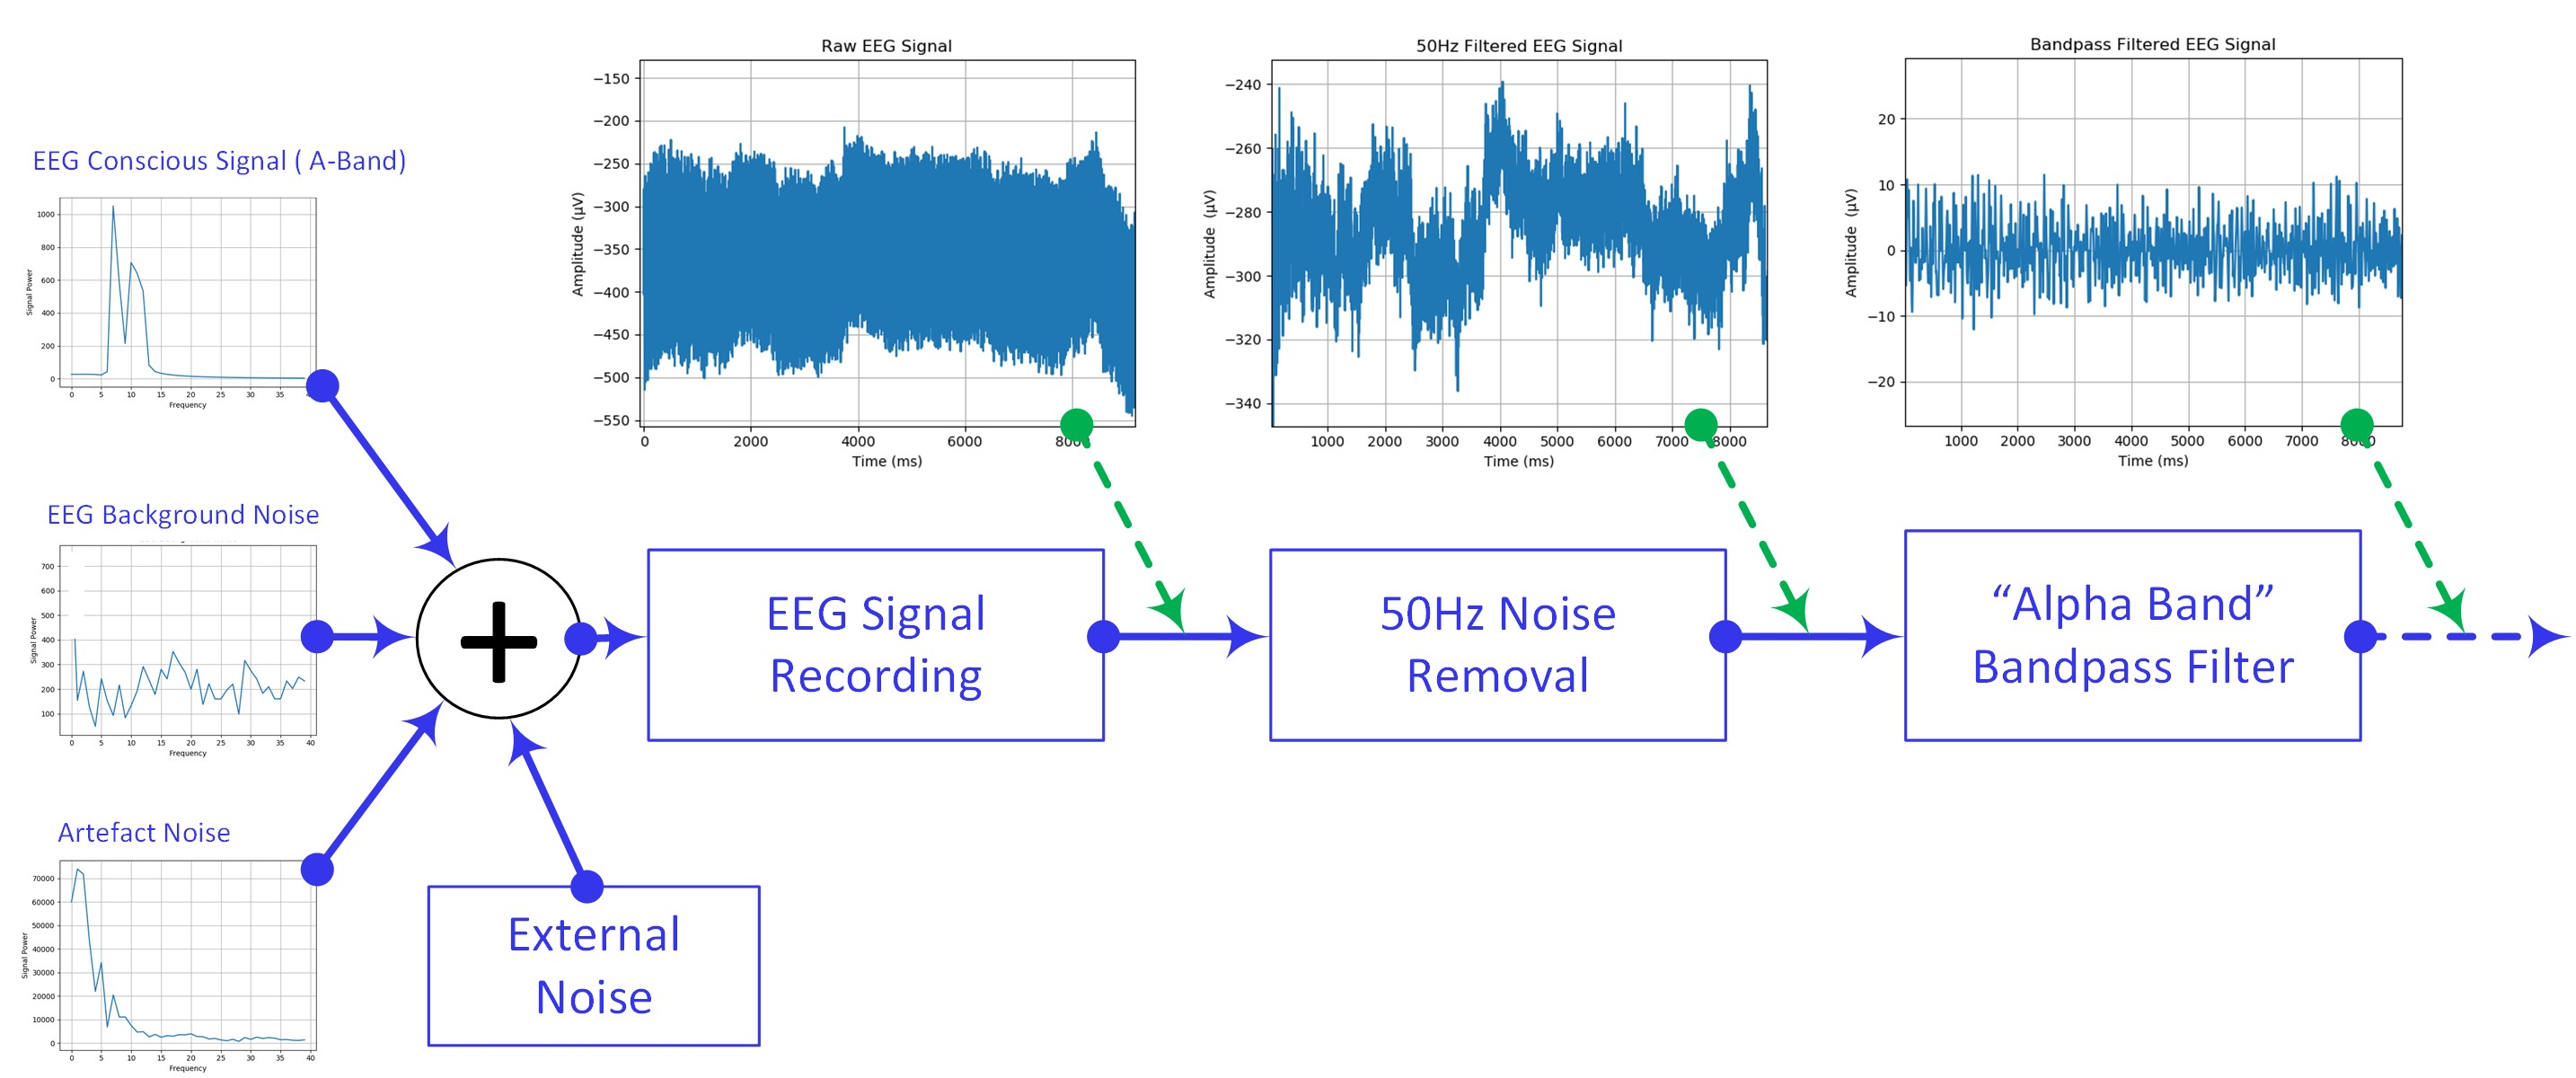
\includegraphics[width=\linewidth]{Figures/EEGsignals.jpg} 
%	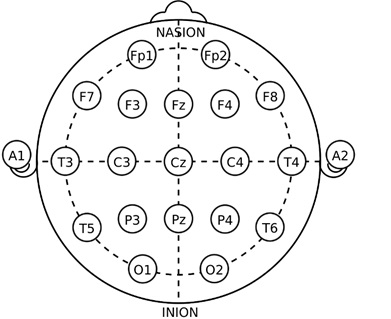
\includegraphics[width=8cm]{Figures/Brain_I20.jpg} 
	\caption{EEG Signals and Preprocessing} 
	\label{EEGsignals} 
\end{figure}





 In the sample domain, a clean EEG recording can be expressed with Equation \ref{eeg_signal}, where M represent the recorded clean EEG signal.In   Equation  \ref{eeg_signal} the components A[n] and B[n] correspond to noise and their sum can be represented with R[n]. 

\begin{equation}
M[n]=A[n]+B[n]+C[n] = R[n]+C[n]
\label{eeg_signal}
\end{equation}


To be able to determine the SNR it is essential to specify which component of the EEG recording is considered to be the noise and which the signal. In \citep{Repovs2010} for the calculation of the SNR, noise was considered to be the EEG component recorded during an artefact, while signal was the consciously generated signal. This is reasonable, since the purpose of the corresponding work was related to the SNR during artefact occurrence. In \citep{Porr2018}, in order to calculate the noise wall, the background noise, EEG signal when the subject is relaxed, was considered to be the minimum noise, while the maximum noise was the mean of all occurrences of artefact noise. The minimum and the maximum noise values were used to calculate the uncertainty (\textrho) of the noise, which in the basis for the calculation of the SNR wall. For the calculation of the SNR, the noise power was considered to be the noise uncertainty multiplied by the minimum noise variance, while the signal power was the consciously generated signal power of paralyzed subject.

The work of this project is different from the work in \citep{Porr2018}  since the aim now is to compute the SNR for EEG signals recorded during motor imagery activities that is, when the subject concentrates on performing a mental activity, and then compare the SNR with the SNR wall to determine if a safe detection can be made.   To this end:
\begin{enumerate} [label=\alph*)]

	\item The subjects are instructed to avoid any body activities that result in artefact noise. 
	\item The subjects are instructed to remain relaxed for a few seconds at the beginning of each experiment. As in \citep{Porr2018} the recorded signal for this time period corresponds to the background noise B[n]. After this time interval, the subject concentrates on carrying out a mental task. The recorded signal for this time interval correspond to the signal component C[n]. Therefore, it is not necessary to use the EEG signals from a paralysed subject.
	\item The calculation of the SNR will be based on the ratio of the variance of the signal component C[n] to the variance of the noise component B[n]. Any artefacts during the EEG recording will contaminate either the noise component, or the signal component, or both, according to the time of occurrence of the artefact. For this study, multiple EEG recordings were obtained. The time plot of these recordings were examined in order to check if the signal contains signal level fluctuations due to artefact. In the case that a non-intentional artefact was identified in a recording, then the EEG recording was discarded. However, there is no quarantine that the rest of the EEG recordings are completely free from artefacts.

\end{enumerate} 

As described in part (b) above, the noise component B[n] and the conscious signal component C[n] will be obtained from different time intervals in the EEG recording. Artefact signals are non-stationary, in the sense that they don’t behave the same way at all times. For example, an artefact might occur due to a non-intentional eye movement during the period of recording the relax signal only. Since the SNR is computed using EEG signals recorded during different time periods, Equation \ref{eeg_signal} can be re-written as shown in Equation  \ref{eeg_signal2}. 


\begin{equation}
M[n]=(B[n]+A_1 [n])+(C[n]+A_2 [n])
\label{eeg_signal2}
\end{equation}

For the purpose of this work, it is assumed that the recorded EEG signals are free from artefacts, therefore the components A1[n] and A2[n] are equal to zero.  Background EEG noise exists in all frequencies of the EEG, while motor imagery brain activities affect only specific frequencies. Therefore, to calculate the SNR it is essential that the EEG signal is bandpass filter in order to isolate the frequency band of interest. The filter signal D[n] is given by Equation \ref{eeg_filter1}, where F[n] is the transfer function of the filter. Equation  \ref{eeg_filter1} can be writen as shown in Equation  \ref{eeg_filter2}, where N[n] is the filtered noise signal and S[n] is the filtered conscious signal. 


\begin{equation}
D[n]=(B[n]+C[n])*F[n]
\label{eeg_filter1}
\end{equation}


\begin{equation}
D[n]=B[n]*F[n]+C[n]*F[n]=N[n]+S[n]
\label{eeg_filter2}
\end{equation}

The SNR can be computed by dividing the variance of the signal with the variance of the noise, as shown in Equation \ref{snr1} and then converted to decibels, if necessary. 


\begin{equation}
SNR = \frac{Signal Power}{Noise Power} = \frac{\sigma_{S}^2 }{\sigma_{N}^2 }
\label{snr1}
\end{equation}

As stated in the Experiment Procedure (Section 3.2), a number of experiments will be conducted where the noise signal is assumed to be the EEG signal obtained when the subject is relaxed. It is expected that for a given subject the noise signal must not change. To ensure a more accurate figure for the noise, the mean of the noise measured between all experiments can be used. Another way to view this is through the noise uncertainty factor (\textrho), a factor that specifies how the noise of a subject is expected to change. Since each subject will carry out a number of experiments, with the background noise recorded at the beginning of the experiment when the subject is relaxing, the maximum and the minimum noise variances between the different experiments can be used to compute the noise uncertainty, according to Equation \ref{rho}.

\begin{equation}
Noise  Uncertainty:  \rho = \sqrt{\frac{\sigma_{Rmax}^2 }{\sigma_{Rmin}^2 }}
\label{rho}
\end{equation}

Where:  $\textsigma_{Rmax}^2$ is the maximum noise variance between the different experiments. 

\hspace{12mm} $\textsigma_{Rmin}^2$ is the minimum noise variance between the different experiments.
 
The noise variance based on the noise uncertainty can be computed using  Equation \ref{noiseV},  while the SNR can now be computed using  Equation \ref{snr2}.

\begin{equation}
Noise  Variance: \sigma_{R,n}^2 = \rho * \sigma_{Rmin}^2 
\label{noiseV}
\end{equation}

\begin{equation}
SNR =  \frac{\sigma_{C}^2 }{\sigma_{R,n}^2 }
\label{snr2}
\end{equation}


\subsection{\bf{Data Analysis Method:}}
This section describes the steps needed in order to determine the SNR wall for each subject, calculate the SNR for each experiment and determine if it is possible to detect the EEG signal. The steps needed are the following:
\begin{description}
 	\item[Step1: ] Filter the EEG signal to remove any external noise such as the 50Hz mains noise.
	\item[Step2: ] Band-pass filter the EEG recording to remove all frequencies except the alpha band frequencies (8Hz to 12Hz). 
	\item[Step3: ] 	For each subject isolate the first part of the recording of each experiment that corresponds to the relaxing period. Calculate the noise variance for each experiment. Find the maximum and the minimum noise variances. ($\textsigma_{Rmax}^2$) and ($\textsigma_{Rmin}^2$).
	\item[Step4: ] For each subject use Equation \ref{rho} to calculate the noise uncertainty (\textrho). Use Equation \ref{noiseV} to calculate the noise variance ($\textsigma_{R,n}^2$) for each subject. 
	\item[Step5: ] For each subject and each experiment calculate the conscious signal variance  $\textsigma_{C}^2$ for the samples corresponding to the first second of the conscious activity of the subject. Use Equation \ref{snr2} to determine the SNR. Repeat for the next segment of the EEG signal. The distance between adjacent segments is 500ms. 
	\item[Step6: ] For each subject and each experiment compare the SNR wall from  \citep{Porr2018} and the SNR from step 5 to determine if a safe detection can be made.  
  
\end{description}

